\chapter{2st class }

Let's define the following differential equation 

\begin{equation}
	Lu = f
\end{equation}

where the linear operator $Lu$ is defined as 
\begin{equation}
	Lu = -u''
\end{equation}

 and using the Laplacian or Laplace operator
 
\begin{equation}
Lu = - \laplacian{u} = - \Delta u
\end{equation}

A boundary-value problem can be defines then as

\begin{equation}
\label{example1}
\begin{split}
- \Delta u & = 1 \\
u & = 0  \quad  x \in \partial{\Omega}
\end{split}
\end{equation}

where  the domain is define 
\begin{equation}
\Omega = (0,1) \times (0,1) - (\sfrac{1}{2},1) \times (\sfrac{1}{2},1) 
\end{equation}

graphically, 

 \begin{center}
	\rotatebox{0}{
		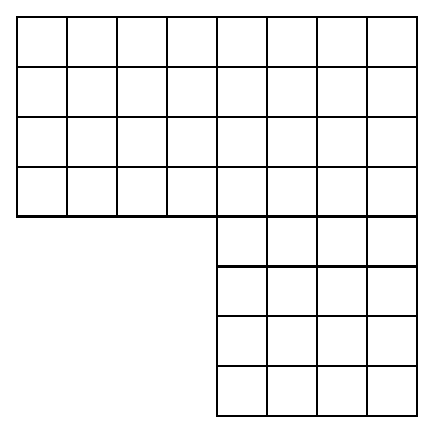
\includegraphics[width=4cm]{images2/discretization.eps}}
\end{center} 

and the task is to approximate \eqref{example1} by polynomials $\in C^2$ or differentiable up to second derivative. This is a minimization problem, where it can be used LSM 

\begin{equation}
S(u) = \int_{\Omega} (Lu - f)^2 \rightarrow min
\end{equation}

or RITZ method based on minimize the energy of the system as follows

\begin{equation}
E(u) = \int_{\Omega} Lu\cdot u - 2fu  \rightarrow min
\end{equation}

Defining a space $V$ where  $V_n \subset V$ and $V_n = \zeta_{exp}(\varphi_1, \varphi_2, ..., \varphi_n)$ where $\varphi_n$ is a polynomial of degree n, and $dim(V_n) < n$, and the approximate solution of the differential equation is 

\begin{equation}
u_n = \sum_{i=1}^{n} \alpha_i \varphi_i
\end{equation}

The energy of the system is defined as

\begin{equation}
E(u_n) = \int_{\Omega}\left(  L \sum_{i=1}^{n} \alpha_i \varphi_i\right)  \sum_{j=1}^{n} \alpha_j\varphi_j - 2f  \sum_{i=1}^{n} \alpha_i \varphi_i 
\end{equation}

\begin{equation}
E(u_n) = \int_{\Omega}  \sum_{i=1}^{n} \sum_{j=1}^{n}  \alpha_i  \alpha_j L  \varphi_i \varphi_j - 2 \sum_{i=1}^{n} \alpha_i f \varphi_i 
\end{equation}

\begin{equation}
E(u_n) =  \sum_{i=1}^{n} \sum_{j=1}^{n}  \alpha_i  \alpha_j \int_{\Omega}   L \varphi_i \varphi_j - 2 \sum_{i=1}^{n} \alpha_i \int_{\Omega}  f \varphi_i 
\end{equation}

In matrix form

\begin{equation}
E(u_n) = \alpha^T \mathbf{A} \alpha - 2 \alpha^T b
\end{equation}

where 

\begin{equation}
A_{ij} = \int_{\Omega}   L \varphi_i \varphi_j 
\end{equation}
 
 and 
 
 \begin{equation}
 b_{i} = \int_{\Omega}  f \varphi_i
 \end{equation}


We will defined $u_{n1}, u_{n2}, ..., u_{nn}$ but the question is $$\lim_{i\to\infty }u_{ni}$$ exist or not, since there can be smooth functions where the limit is not part of the same space $V$. 

The space $V$ is defined as  $\norm{\cdot}$: $V \rightarrow  \real_0^+$ with the following properties

\begin{enumerate}
	\item  $\norm{u} \geq 0$
	\item  $\norm{u} = 0  \quad u=0$
	\item  $ \norm{\alpha u} = \alpha \norm{u}$
\end{enumerate}

Def: \\
$\lim u_{n} = u$ $\leftrightarrow \forall \varepsilon > 0 \quad  \exists n_0 \quad \forall n >n_0 : \quad \norm{u-u_n} < \varepsilon$

 \begin{center}
	\rotatebox{0}{
		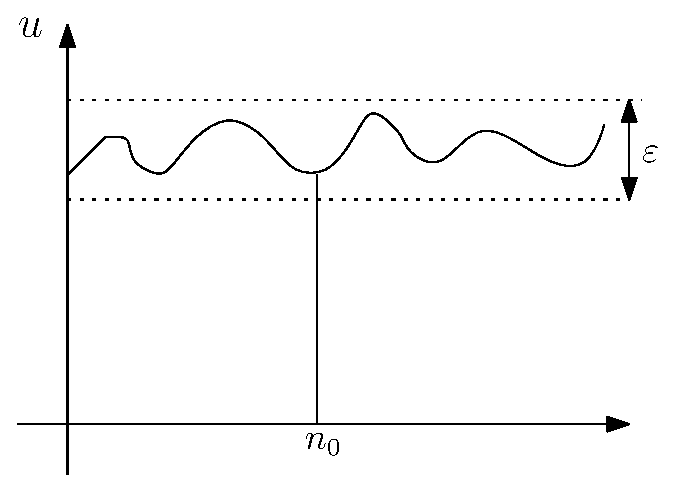
\includegraphics[width=4cm]{images2/derivative.eps}}
\end{center} 

The more common norms are $\norm{\cdot}_p$ and $\norm{\cdot}_\infty$, defined as follows for $V= C_{<0,1>}$
\begin{equation}
	\begin{split}
		\norm{u}_\infty & =   \max_{x\in(0,1)}\abs{u(x)} \\
		\norm{u}_p & = \left( \int_{0}^{1} \abs{u(x)}^p\right)^{\frac{1}{p}}
	\end{split}
\end{equation}

Def: \\
$u_n$ is cauchy $\leftrightarrow \forall \varepsilon > 0 \quad  \exists n_0 \quad \forall n,m >n_0 : \quad \norm{u_n-u_m} < \varepsilon$

any convergent sequence is cauchy but not every cauchy sequence is convergent. 

If we defined $\bar{V} = \bar{\bar{V}}$ is a closed space of $V$ where we add all the cauchy sequences, named $H_1$. $H_1$ is a space that can contain continuous but not smooth function. In other words, there are functions that do not have second derivative.  Notice then, for  $v \in H_1$ , $Lv = f $ is not satisfy. 

The Galerkin method states 
\begin{equation}
	\forall v \quad (Lu,v) = (f,v)
\end{equation}

Assuming homogeneous Dirichlet condition $u(0)=u(1)=0$, we have

\begin{equation}
\int_{0}^{1} (-(pu')' + qu)\cdot v = \int_{0}^{1} f\cdot v
\end{equation}

Proceeding with  integration by parts

\begin{equation}
\int_{0}^{1} -(pu')v' + quv  = \int_{0}^{1} f\cdot v
\end{equation}

\begin{equation}
\int_{0}^{1} (-(pu')' v +\int_{0}^{1} qu v =   - pu'v \Big|_0^1  +   \int_{0}^{1} pu'v' + \int_{0}^{1} fv
\end{equation}
	
\begin{equation}
  \int_{0}^{1} pu'v' + qu v  =  \int_{0}^{1} fv
\end{equation}

which is equivalent to the weak form 

\begin{equation}
(u,v)_L = (f,v)
\end{equation}

The weak solution is not related to the original problem, moreover, notice it is no longer required continuity in the second derivative since $u''$  is not par of the solution. 